\section{ Data Warehouse}
\subsection{O que é um Data Warehouse}
Para \citeAuthorPageYear{jmj}, um \textit{Data Warehouse} é um repositório de informações coletadas de múltiplas fontes, armazenado sobre um esquema definido e, geralmente, situado em um único local, no intuito de garantir a consistência dos dados caso eles sejam acessados de locais diferentes. Eles suportam o processamento de informações ao prover uma plataforma sólida de dados históricos para análise \citep{jmj}.

\subsection{Características de um Data Warehouse}
Segundo \citeAuthorPageYear{inmon}, um DW (Data Warehouse) é um conjunto de dados orientado por assuntos, integrado, variável com o tempo e não volátil, criados para dar suporte à decisão.

Orientado por assunto, ou seja, organizado em torno de um assunto principal. Em vez de se concentrar nas operações diárias e no processamento de transações de uma empresa, um DW foca na modelagem e análise de dados para tomadores de decisões \citep{jmj}.
Integrado, um DW contém informações de fontes heterogêneas, como base de dados relacionais e \textit{flat files}. Processos de \textit{data integration} e \textit{data cleaning} são aplicados para garantir a consistência dos dados.

Variável com o tempo, armazena informações históricas dos últimos 5-10 anos, por exemplo. Toda estrutura chave em um DW contém um elemento de tempo \citep{jmj}.
E por último, não volátil, os dados não precisam ser alterados, já que um DW é fisicamente separado do ambiente operacional. As únicas operações executadas em um DW são: carga inicial e acesso aos dados \citep{jmj}.

\subsection{Modelos de Data Warehouse}
Para \citeAuthorPageYear{jmj}, um DW pode ser dividido em três modelos: \textit{enterprise warehouse}, \textit{data mart} e \textit{virtual warehouse}.

\subsubsection{Enterprise Warehouse}
\citeAuthorPageYear{jmj} diz que um \textit{enterprise warehouse} coleta informações sobre um assunto que abrange toda uma organização. Ele fornece integração de dados em escala corporativa, geralmente de um ou mais sistemas operacionais ou de provedores de informação externos. Ele contém dados detalhados e sumarizados e podem variar de alguns poucos \textit{gigabytes} para centenas de \textit{gigabytes}.

Um \textit{enterprise warehouse} é um conglomerado das \textit{data warehouse staging} e \textit{presentation areas} de uma organização \citep{kimball2002}


\subsubsection{Data Mart}
Conforme \citeAuthorPageYear{jmj} diz, um \textit{data mart} contém um subconjunto de dados de uma escala corporativa e tem o escopo limitado a assuntos específicos.

Os \textit{data marts} são frequentemente implementados em servidores de baixo custo e têm o seu ciclo de implementação medido em semanas, em vez de meses ou anos. Os dados podem ser independentes ou dependentes. Caso sejam independentes, vão ter como fonte um ou mais sistemas operacionais ou provedores de informação externos. No caso de serem dependentes, os dados contidos no \textit{data mart} serão fornecidos diretamente de um \textit{enterprise warehouse}.

\subsubsection{Virtual Warehouse}
\citeAuthorPageYear{jmj} dizem que as \textit{virtual warehouses} são um conjunto de \textit{views} em cima dos bancos de dados operacionais. Eles podem manter um processamento eficiente de \textit{queries} exibindo apenas alguns dos possíveis sumários. Ele também é de fácil construção.

\subsection{Componentes}

A figura \ref{dwComponents} mostra quais são os componentes de um DW, explicados com detalhes mais abaixo.
\begin{figure}[H]
\centering
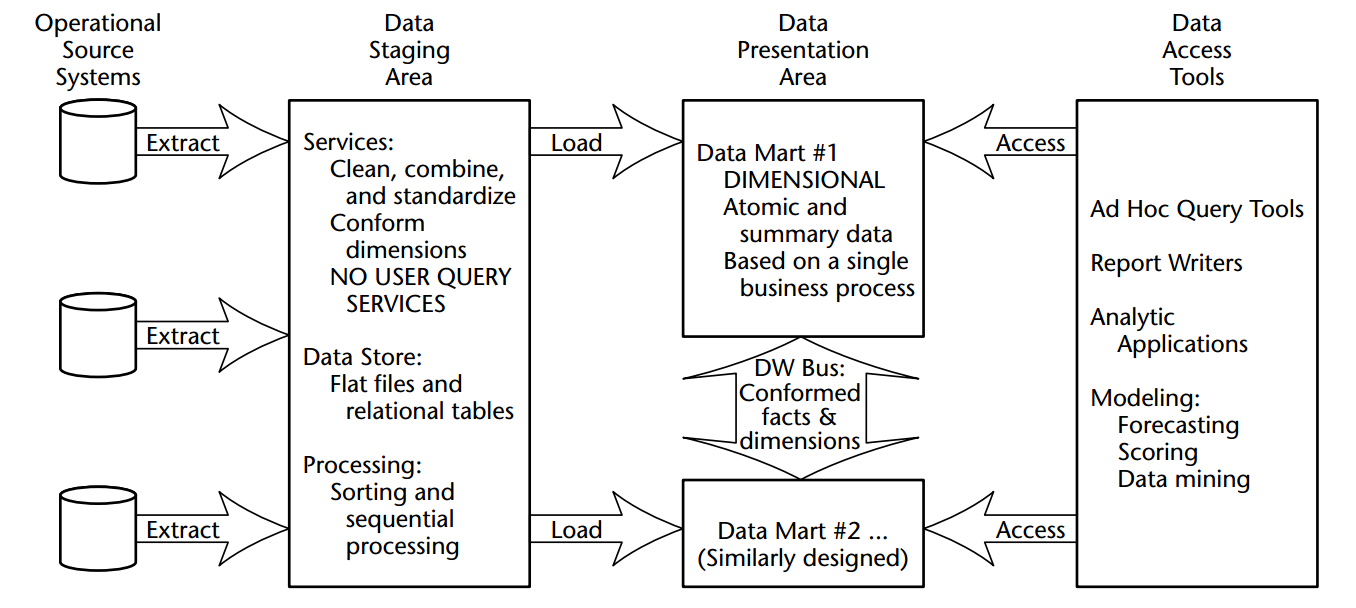
\includegraphics[height=5cm]{imagens/componentes_DW.png}
\caption{Componentes de um Data Warehouse (\citeauthor{kimball2002} \citeyear{kimball2002})}
\label{dwComponents}
\end{figure}

\subsubsection{Operational Source Systems}
Fontes de Dados Operacionais, nas palavras de \citeAuthorPageYear{kimball2013}, são responsáveis pela captura de transações de negócio. Esses sistemas são mantidos fora do \textit{data warehouse} porque se tem pouco ou nenhum controle sobre o conteúdo ou formato dos dados. Eles processam performance e disponibilidade. Eles também afirmam que esses sistemas mantêm poucos dados históricos. Um bom \textit{data warehouse} pode reduzir a necessidade dos sistemas de dados operacionais de representarem o passado. Em muitos casos, eles são de algum propósito especial, sem responsabilidade de compartilhar dados comuns, como dados de produtos, clientes etc.

\subsubsection{Data Staging Area}
\citeAuthorPageYear{kimball2002} sugerem que a \textit{staging area} é tanto uma área de armazenamento como um conjunto de processos conhecidos como \textit{extract, transformation, loading} (ETL). Esse processo será melhor explicado mais pra frente. Eles ainda falam que a \textit{staging area} é tudo entre os \textit{operational source systems} e a \textit{presentation area}. 

Existem diversas formas de carregar dados na \textit{staging area}, como \textit{flat files}, xml, modelos relacionais. Ela regularmente é composta de um \textit{database management system} (DBMS) e arquivos de texto (\textit{flat files}) \citep{kimball2004}. Em muitos casos, os dados precisam ser armazenados fora de um DBMS, em \textit{flat files}, para um rápido processamento sequencial.
\citeAuthorPageYear{kimball2002} descrevem o primeiro passo na criação (extração) de um \textit{data staging area} como ler e entender da fonte de dados e copiar o que for necessário para manipulação futura. Afirma que quando os dados são extraídos, existem diversas transformações que podem ser feitas, como limpeza, combinação de dados de diferentes fontes, remoção dados duplicados etc. Essas transformações acontecem antes de se carregar os dados na \textit{presentation area}.

\subsubsection{Data Presentation Area}
A \textit{presentation area}, ou área de apresentação, é onde os dados estão organizados, armazenados e disponíveis para consulta por usuários ou alguma aplicação analítica de \textit{Business Intelligence} (BI) \citep{kimball2013}. Tudo que o negócio vê e toca é através das ferramentas de acesso ou aplicações de BI.

Os dados devem ser, de acordo com \citeAuthorPageYear{kimball2013}, apresentados, armazenados e acessados através de esquemas dimensionais, sejam eles esquemas estrela ou cubos OLAP (\textit{online analytical processing cubes}), que são modelos dimensionais de alta performance implementados em \textit{softwares} de proposito especial. Eles devem conter dados atômicos detalhados. Embora a \textit{presentation area} contenha dados agregados, é completamente inaceitável que somente dados sumarizados sejam armazenados enquanto os dados atômicos estão trancados em modelos normalizados. Os dados mais finamente granulados devem ser apresentados na \textit{presentation area} para que usuários possam fazer as perguntas mais precisas.

A área de apresentação deve ser estruturada ao redor dos processos de medição de eventos. Os modelos dimensionais devem corresponder aos eventos de captura de dados, não devem entregar um "relatório do dia" \citep{jmj}. 

\subsubsection{Data Access Tools} Ferramentas de Acesso de Dados, ou \textit{Data Access Tools}, são ferramentas usadas para consultar área de apresentação. Uma ferramenta dessas pode ser tão simples quanto \textit{Queries Ad Hoc}, \textit{queries} usadas para determinado proposito e usadas quando se tem a necessidade, ou tão complexa quanto uma ferramenta de mineração de dados ou modelagem \citep{kimball2013}. 

\subsection{Extract, Transform, Load (ETL)}
O processo de \textit{extract, transform, load} (extrair, transformar, carregar), mais conhecido como ETL, é um processo utilizado para a construção de um DW, contendo os passos que são mostrados na figura \ref{etl}. 
\begin{figure}[H]
\centering
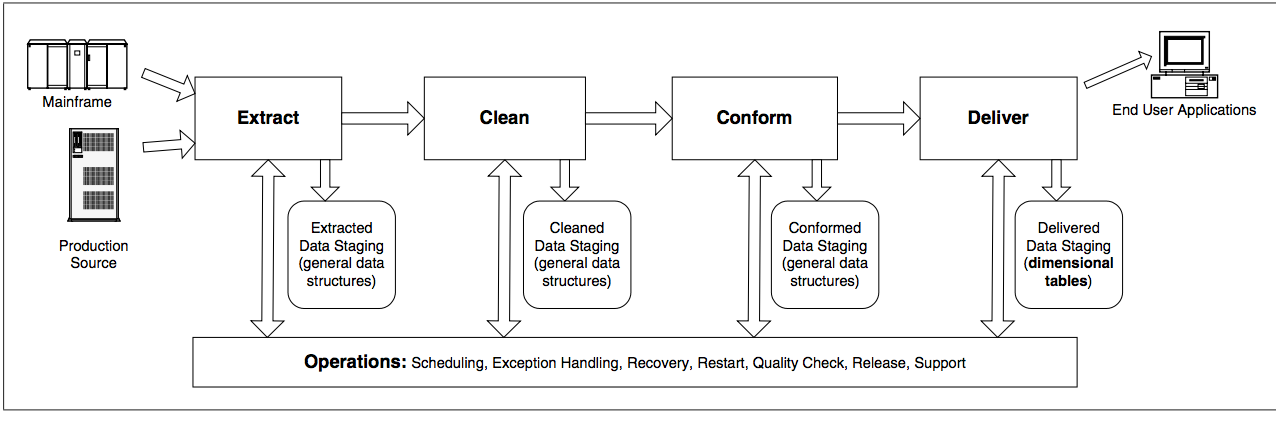
\includegraphics[height=5cm]{imagens/dw_process.png}
\caption{Processo de ETL (\citeauthor{kimball2004} \citeyear{kimball2004})}
\label{etl}
\end{figure}
O primeiro passo é a extração dos dados: espera-se que o sistema extraia dados de uma grande variedade de fontes \citep{kimball2013}. As organizações podem extrair dados de fontes como arquivos xml, banco de dados, planilhas etc.

O segundo passo é a transformação: após os dados serem extraídos, diversas transformações podem ser executadas, como limpeza, que irá remover alguns ruídos, combinação de dados de fontes diversas (bancos de dados, \textit{data warehouses}, arquivos csv, planilhas, etc) e tratar dados duplicados\citep{kimball2013}. Essa limpeza pode mudar os dados e aperfeiçoar o seu valor para uma organização.

O terceiro e último passo é o carregamento, que é o processo de estruturar fisicamente e carregar os dados dentro dos modelos dimensionais da \textit{presentation area} \citep{kimball2013}.

\subsection{Modelagem Dimensional}
A modelagem dimensional permite que os usuários do negócio enxerguem os dados com facilidade, ao entregar dados entendíveis e uma performance rápida, com dados visualizados em dimensões.

Existem quatro etapas para a construção de um modelo dimensional, sendo elas: \textbf{selecionar o processo de negócio}, \textbf{declarar o grão}, \textbf{identificar as dimensões} e \textbf{identificar os fatos}. 

Segundo \citeAuthorPageYear{kimball2013}, os processos de negócio são as atividades operacionais realizadas por uma organização. É um processo importante, pois define como o grão, dimensões e fatos serão declarados. O grão estabelece o que uma única linha na tabela de fatos representa.

\subsubsection{Tabela de Dimensões}
De acordo com \citeAuthorPageYear{kimball2013}, as dimensões fornecem o contexto de "quem, o que, onde, quando e como" de cada processo do negócio. As tabelas de dimensões podem incluir diversas colunas, mas costumam ter menos dados que a tabela de fatos. Elas têm chave primária, que vai permitir o relacionamento com a tabela de fatos.
A tabela de dimensões pode ser conhecida como a "alma" de um sistema de DW, pois contém dados que permitem que o sistema de DW seja alavancado.

\subsubsection{Tabela de Fatos}
A tabela de fatos armazena as métricas resultantes de um processo de negócio de uma organização \citep{kimball2013}. Cada linha em uma tabela de fatos representa um evento de medição. Os dados, em um nível especifico de detalhe, podem ser chamados de grãos, como apenas uma linha por produto vendido.

Os dados mais úteis são os numéricos e aditivos. Aditividade é importante, pois dificilmente irá se fazer uma consulta que traga apenas uma linha, mas sim trará centenas, milhares ou milhões de dados e a coisa mais útil para se fazer com eles é somar \citep{kimball2013}.

\citeAuthorPageYear{kimball2013} falam que é possível manter dados textuais em uma tabela de fatos, eles são comumente usados para descrever algo e estão em uma lista discreta de valores. 

As tabelas de dimensões, conforme \citeAuthorPageYear{kimball2013}, têm uma ou mais chaves estrangeiras, que irá se ligar as chaves primarias das tabelas de dimensões. Eles afirmam que a tabela de fatos tem sua própria chave estrangeira, que é um subconjunto das chaves estrangeiras, chamado de chave composta. 

\subsubsection{Esquema Estrela}
Esse esquema, mostrado como exemplo na figura \ref{star}, armazena os dados em uma arquitetura semelhante a uma estrela, onde cada ponta é uma dimensão e todas se relacionam com a tabela de fatos, como mostra a figura. \citeAuthorPageYear{jmj} mostram que a tabela de fatos contém chaves para todas as outras tabelas assim como dados de medidas.
\begin{figure}[ht]
\centering
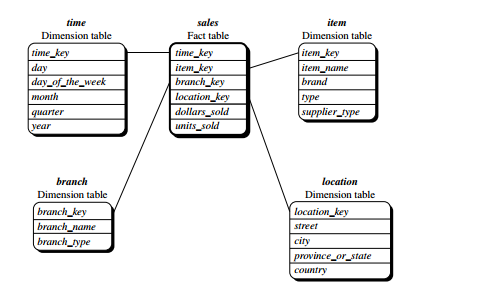
\includegraphics[height=6.2cm]{imagens/starscheme.png}
\caption{Esquema Estrela (\citeauthor{jmj} \citeyear{jmj})}
\label{star}
\end{figure}
\\
\subsubsection{Esquema Snowflake}
Como mostra na figura \ref{snowflake}, o esquema \textit{snowflake} é uma variação do esquema estrela onde algumas tabelas de dimensões são normalizadas, ou seja, dividindo os dados em tabelas adicionais \citeAuthorPageYear{jmj}.
\begin{figure}[ht]
\centering
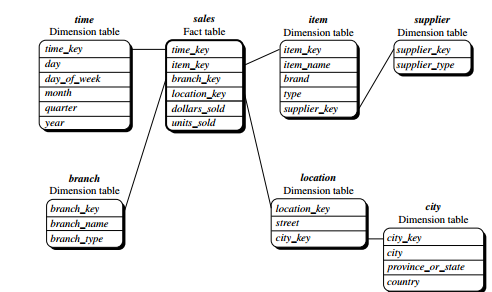
\includegraphics[height=6.2cm]{imagens/snowflakescheme.png}
\caption{Esquema Snowflake (\citeauthor{jmj} \citeyear{jmj})}
\label{snowflake}
\end{figure}
\subsubsection{Cubo e OLAP}
Conforme \citeAuthorPageYear{jmj}, DW e ferramentas OLAP são baseados no modelo multidimensional e ele visualiza os dados no formato de cubos de dados, como mostra a figura \ref{cube}. Um cubo permite visualizar os dados em diversas dimensões simultaneamente.
\begin{figure}[ht]
\centering
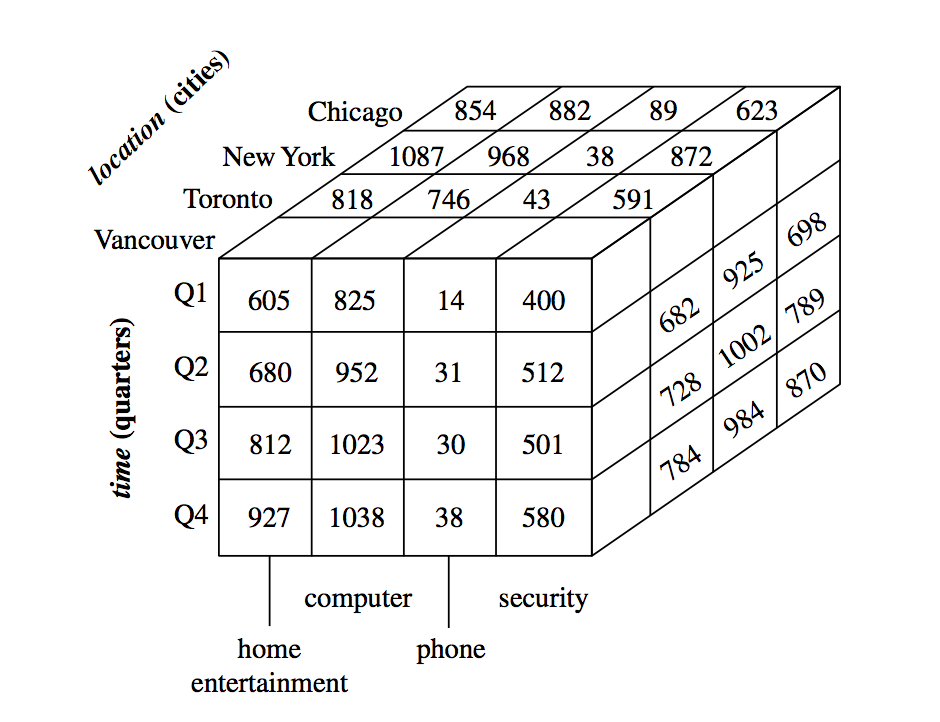
\includegraphics[height=6.2cm]{imagens/datacube.png}
\caption{Exemplo de um cubo de dados (\citeauthor{jmj} \citeyear{jmj})}
\label{cube}
\end{figure}
Dimensões são entidades que uma organização quer manter os dados. Uma dimensão deve ter uma tabela associada, a tabela de dimensões.


\citeAuthorPageYear{kimball2013} dizem que os modelos dimensionais implementados em base de dados multidimensionais são chamados de \textit{online analytical processing cubes} (OLAP). Diversas operações estão associadas a esses cubos, como \textit{roll up, drill down, slice and dice e pivot}

\begin{itemize}
    \item \textbf{roll-up}: segundo \citeAuthorPageYear{jmj}, a operação de \textit{roll-up} executa agregações em um cubo de dados ou por \textit{subir em uma hierarquia conceitual} de uma dimensão ou por redução dimensional. Quando essa operação é realizada, uma ou mais dimensões podem ser retiradas do cubo.
    
    \item \textbf{drill-down}: Essa operação é a inversa da \textit{roll-up}, indo de dados menos detalhados para dados mais detalhados. Pode ser feito ou por \textit{descer uma hierarquia conceitual} de dimensões ou \textit{introduzir dimensões adicionais} \citep{jmj}
    
    \item \textbf{slice and dice}: A operação \textbf{slice} faz uma seleção em uma subdimensão do cubo, resultando em um subcubo \citep{jmj}. A operação \textbf{dice} cria um subcubo ao efetuar uma seleção em uma ou mais dimensões \citep{jmj}.
    
    \item \textbf{pivot}: \citeAuthorPageYear{jmj} dizem que \textit{pivot} (ou rotate) é uma operação que permite mover o cubo em algum eixo permitindo uma exibição dos dados em de uma forma alternativa.
\end{itemize}
